%==============================================================================
% Sjabloon poster bachproef
%==============================================================================
% Gebaseerd op document class `a0poster' door Gerlinde Kettl en Matthias Weiser
% Aangepast voor gebruik aan HOGENT door Jens Buysse en Bert Van Vreckem

\documentclass[a0,portrait]{hogent-poster}
\usetikzlibrary{positioning}
\usepackage{colortbl}
\usepackage[export]{adjustbox}

% Info over de opleiding
\course{Bachelorproef}
\studyprogramme{toegepaste informatica}
\academicyear{2025-2026}
\institution{Hogeschool Gent, Valentin Vaerwyckweg 1, 9000 Gent}

% Info over de bachelorproef
\title{Competentieframework voor z/OS System Administrator en System Programmeurs}
\subtitle{Level 1 \& Level 2}
\author{Murat Bugdayci}
\email{murat.bugdayci@student.hogent.be}
\supervisor{Dhr. L. Blondeel}
\cosupervisor{Dhr. J. E. Kok (ABN AMRO)}

% Indien ingevuld, wordt deze informatie toegevoegd aan het einde van de
% abstract. Zet in commentaar als je dit niet wilt.
\specialisation{Mainframe specialist}
\keywords{z/OS besturingsysteem, JCL, REXX, SDSF, RACF, competentieframework}
\projectrepo{https://github.com/muratbugdayc/2026bachelorproefMuratBugdayci}

\begin{document}

\maketitle

\begin{abstract}
De mainframe-sector kampt met een structureel tekort aan gekwalificeerde z/OS-professionals door vergrijzing en een kloof tussen onderwijs en industrie. Deze bachelorproef ontwikkelt een praktijkgericht competentieframework voor z/OS System Administrators en System Programmers (Level 1 \& 2), aangevuld met een proof-of-concept webapplicatie. Via literatuurstudie en semigestructureerde interviews bij o.a.\ ABN AMRO, Euroclear en KBC werden 8 technische en 4 professionele competentiedomeinen geïdentificeerd en gevalideerd.
\end{abstract}

\begin{multicols}{2}

\section{Probleemstelling}

IBM z/OS-omgevingen verwerken wereldwijd meer dan 70\% van de bedrijfskritische transacties bij banken, overheidsinstellingen en verzekeraars. Toch kampt de sector met een structureel personeelstekort: de workforce vergrijst snel en ervaren professionals stromen massaal uit. Tegelijkertijd besteden onderwijsinstellingen nauwelijks aandacht aan mainframe-technologie, waardoor een kloof ontstaat tussen wat studenten leren en wat de industrie verwacht.

\textbf{Onderzoeksvraag:} Welke competenties vereist een z/OS SysAdmin/SysProg, en hoe worden deze georganiseerd in een framework toepasbaar binnen een onderwijscontext?

\section{Methodologie}

\begin{center}
\begin{tikzpicture}[
  node distance=0.8cm and 2.2cm,
  num/.style={circle, draw, fill=hogent-darkgreen, text=white,
              font=\bfseries\normalsize, minimum size=1.1cm, inner sep=0pt},
  card/.style={rectangle, draw=hogent-darkgreen, rounded corners=8pt,
               fill=white, text width=6.8cm, minimum height=3.5cm,
               align=flush left, inner sep=10pt, font=\normalsize}
]

%% Rij 1: drie stappen
\node[card] (c1) {
  \textbf{Literatuur-\\studie}\\[5pt]
  $\bullet$ SFIA, e-CF\\
  $\bullet$ IBM Z Framework\\
  $\bullet$ z/OS stack
};
\node[card, right=of c1] (c2) {
  \textbf{Interviews}\\[5pt]
  $\bullet$ 7 organisaties\\
  $\bullet$ Junior \& senior\\
  $\bullet$ Semigestructureerd
};
\node[card, right=of c2] (c3) {
  \textbf{Ontwikkeling}\\[5pt]
  $\bullet$ Framework\\
  $\bullet$ PoC webappl.\\
  $\bullet$ 25 topics \\
  $\bullet$ IBM Redbooks/docs.
};

%% Genummerde cirkels boven elke kaart
\node[num, above=0.2cm of c1.north] {01};
\node[num, above=0.2cm of c2.north] {02};
\node[num, above=0.2cm of c3.north] {03};

%% Pijlen rij 1
\draw[->, very thick, hogent-darkgreen] (c1.east) -- (c2.west);
\draw[->, very thick, hogent-darkgreen] (c2.east) -- (c3.west);

%% Rij 2: twee stappen gecentreerd onder rij 1
\node[card, below=1.2cm of c3, xshift=-4.6cm] (c4) {
  \textbf{Validatie}\\[5pt]
  $\bullet$ Via literatuur\\
  $\bullet$ Via interviews\\
  $\bullet$ Promotor \& co-prom.
};
\node[card, right=of c4] (c5) {
  \textbf{Framework}\\[5pt]
  $\bullet$ 8 tech.\ domeinen\\
  $\bullet$ 4 prof.\ domeinen\\
  $\bullet$ Level 1 \& 2
};

\node[num, above=0.2cm of c4.north] {04};
\node[num, above=0.2cm of c5.north] {05};

%% Pijl rij 2
\draw[->, very thick, hogent-darkgreen] (c4.east) -- (c5.west);

%% Verbinding rij 1 naar rij 2
\draw[->, very thick, hogent-darkgreen] (c3.south) -- ++(0,-0.6) -| (c4.north);

\end{tikzpicture}
\end{center}

\small\textit{Semigestructureerde interviews met professionals tewerkgesteld bij: KBC, Euroclear, ABN AMRO, Isbank, Halkbank, Planet NL en Broadcom.}\normalsize

\section{Het Competentieframework}

Het framework omvat \textbf{12 domeinen} in twee categorieën, elk uitgewerkt op twee progressieniveaus (Level~1: Basis $\rightarrow$ Level~2: Gevorderd):

\begin{center}
\renewcommand{\arraystretch}{1.4}
\arrayrulecolor{hogent-darkgreen}
\begin{tabular}{|l|l|}
\hline
\rowcolor{hogent-darkgreen}
\multicolumn{2}{|l|}{\textcolor{white}{\textbf{~~Technische Domeinen (T1--T8)}}} \\
\hline
\rowcolor{hogent-darkgreen!15} T1: Platform Fundamentals & T5: Batch Processing \& JCL \\
\hline
\rowcolor{white} T2: Hardware \& Virtualization & T6: Automation \& Scripting \\
\hline
\rowcolor{hogent-darkgreen!15} T3: Storage \& Data Management & T7: Subsystems \& Middleware \\
\hline
\rowcolor{white} T4: System Operations \& Tools & T8: Networking \& Security \\
\hline
\rowcolor{hogent-darkgreen}
\multicolumn{2}{|l|}{\textcolor{white}{\textbf{~~Professionele Domeinen (P1--P4)}}} \\
\hline
\rowcolor{hogent-darkgreen!15} P1: Communicatie \& Samenwerking & P3: Change Management \\
\hline
\rowcolor{white} P2: Probleemoplossing \& Kritisch Denken & P4: Professionele Ontwikkeling \\
\hline
\end{tabular}
\arrayrulecolor{black}
\end{center}

\section{Proof-of-Concept Webapplicatie}

Een statische webapplicatie (GitHub Pages) maakt het framework interactief toegankelijk. Elke competentiekaart bevat theorie, meerkeuzevragen (MCQ) en praktijkopdrachten op basis van realistische z/OS-scenario's. De inhoud van de PoC in cijfers:

\begin{center}
\begin{tikzpicture}[
  stat/.style={rectangle, rounded corners=10pt,
               fill=hogent-darkgreen, text=white,
               text width=4.0cm, minimum height=3.2cm,
               align=center, inner sep=8pt}
]
  \node[stat] at (0,0)    {\textbf{\Large 25}\\[4pt]topics};
  \node[stat] at (5.6,0)  {\textbf{\Large 232}\\[4pt]MCQ-vragen};
  \node[stat] at (11.2,0) {\textbf{\Large 61}\\[4pt]praktijk-\\taken};
\end{tikzpicture}
\end{center}

\begin{center}
\begin{minipage}[t]{0.47\linewidth}
  \captionsetup{type=figure}
  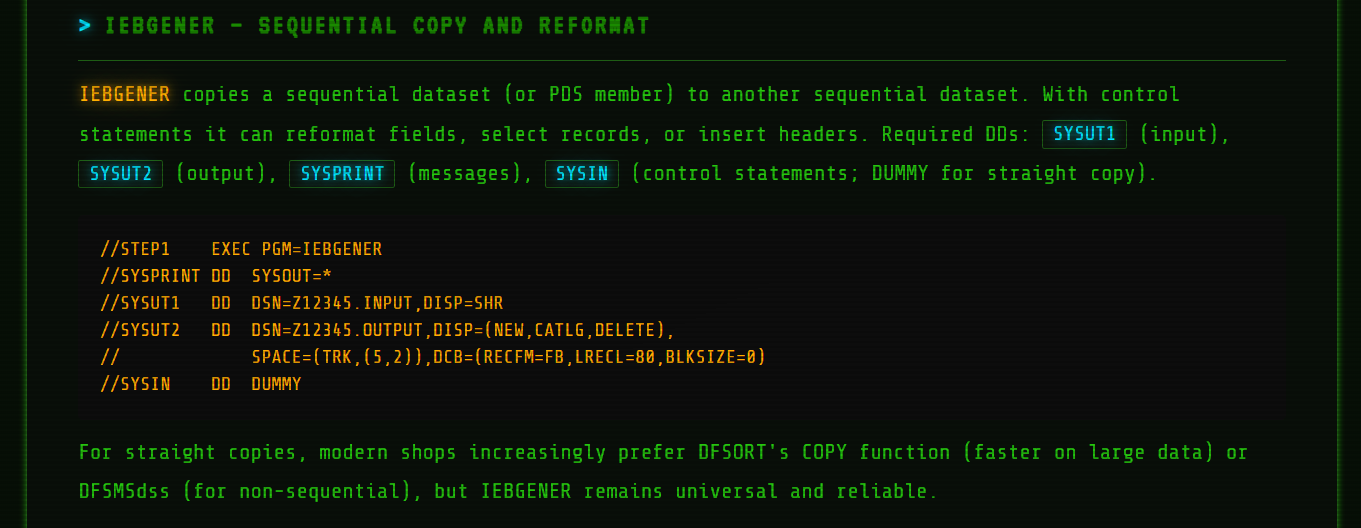
\includegraphics[width=\linewidth, cfbox=hogent-darkgreen 3pt 0pt]{../bachproef/images/BACHPROEFGENER}
  \captionof{figure}{IEBGENER utility (T5: Batch \& JCL)}
\end{minipage}
\hfill
\begin{minipage}[t]{0.47\linewidth}
  \captionsetup{type=figure}
  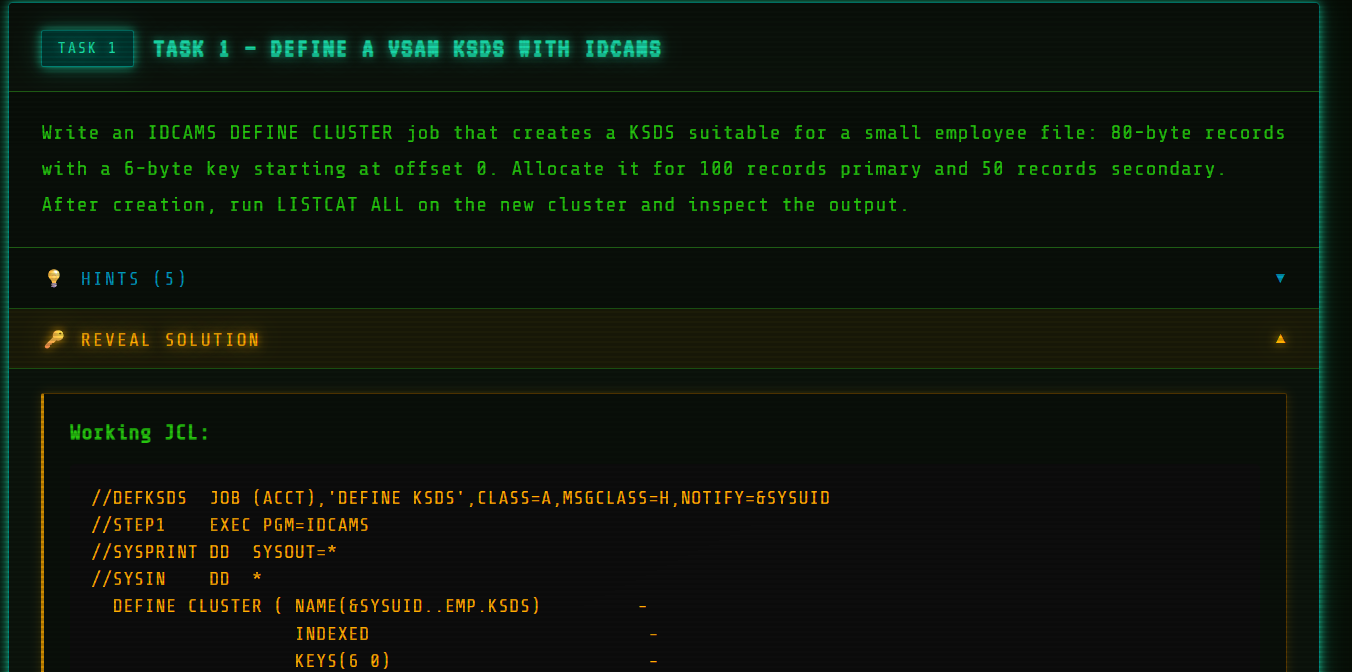
\includegraphics[width=\linewidth, cfbox=hogent-darkgreen 3pt 0pt]{../bachproef/images/BACHPROEFVSAM}
  \captionof{figure}{VSAM KSDS praktijktaak (T3: Storage \& Data Management)}
\end{minipage}
\end{center}

\begin{center}
\begin{minipage}[t]{0.47\linewidth}
  \captionsetup{type=figure}
  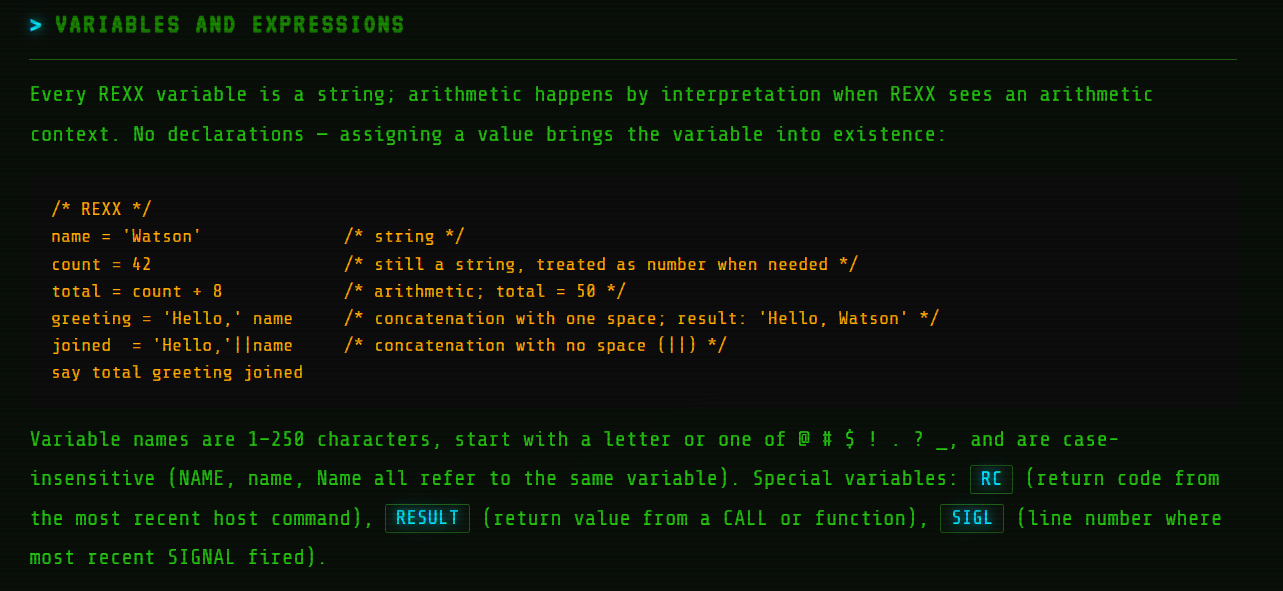
\includegraphics[width=\linewidth, cfbox=hogent-darkgreen 3pt 0pt]{../bachproef/images/bachproefREXX}
  \captionof{figure}{REXX Variables \& Expressions (T6: Automation \& Scripting)}
\end{minipage}
\hfill
\begin{minipage}[t]{0.47\linewidth}
  \captionsetup{type=figure}
  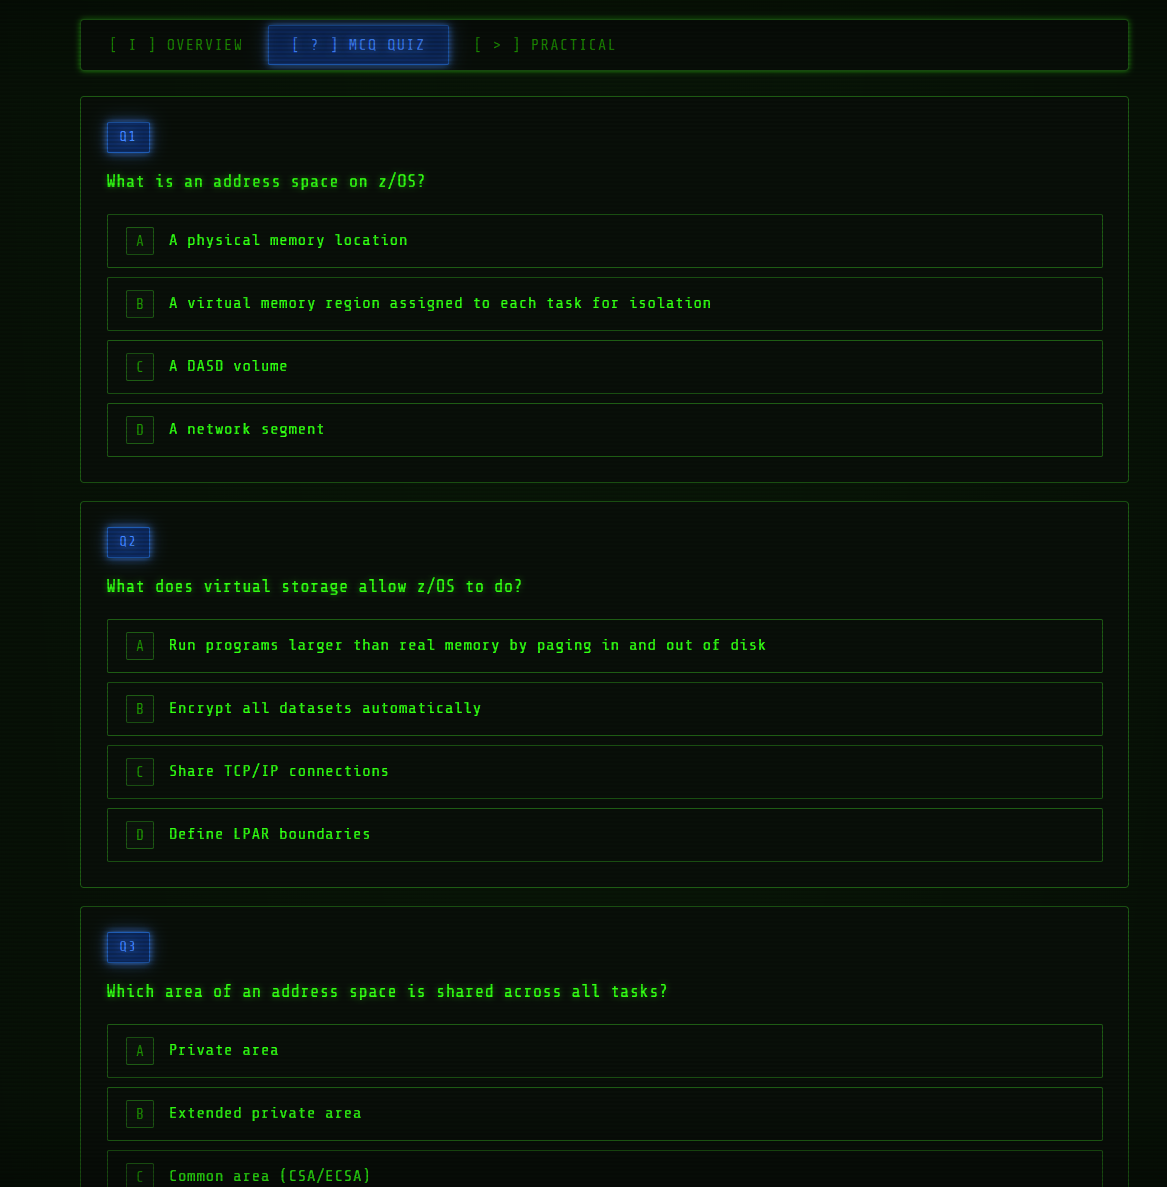
\includegraphics[width=\linewidth, cfbox=hogent-darkgreen 3pt 0pt]{../bachproef/images/bachproef4}
  \captionof{figure}{MCQ-sectie z/OS Overview \& Address Spaces (T1.1)}
\end{minipage}
\end{center}

\section{Conclusies}

\begin{itemize}
  \item \textbf{Rolvervaging:} De grens tussen SysAdmin en SysProg is in de praktijk niet eenduidig en varieert per organisatie; een geïntegreerd framework voor beide rollen is noodzakelijk.
  \item \textbf{Technische prioriteiten:} Abstracte z/OS concepten zoals WLM, Adress spaces en technologieen/talen zoals JCL, TSO/ISPF, SDSF en REXX worden door de meeste van geïnterviewden als kritisch beschouwd voor starters.
  \item \textbf{Soft skills:} Communicatie, probleemoplossend denken en documentatievaardigheid zijn minstens even belangrijk als technische kennis.
  \item \textbf{Meerwaarde PoC:} Professionals bevestigden de waarde van een interactief leerplatform; mainframe-specifiek leermateriaal is schaars.
  \item \textbf{Unieke bijdrage:} Dit framework is specifieker dan SFIA of e-CF doordat het rechtstreeks is afgestemd op z/OS en gebaseerd op industrievalidatie en interviews.
\end{itemize}

\end{multicols}
\end{document}